\chapter{附录A:数据集}

\section{线性可分数据集}

下面的代码用于加载本书大多数章节中使用的简单线性可分数据集。你可以在\href{https://bitbucket.org/syncfusiontech/svm-succinctly}{这里}中找到本书中使用的其他数据集的源代码。

\begin{figure}[ht]
	\centering
	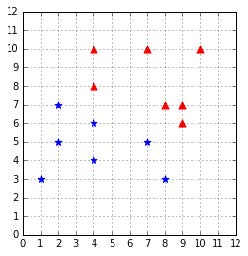
\includegraphics{figure60}
	\caption{训练集}
	\label{figure60}
\end{figure}

\begin{figure}[ht]
	\centering
	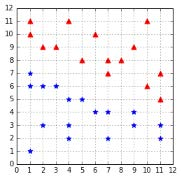
\includegraphics{figure61}
	\caption{测试集}
	\label{figure61}
\end{figure}

当如代码51所示导入模块时,它会加载代码52所示的方法。

方法\colorbox{lightgray}{get\_training\_examples}返回图\ref{figure60}所示的数据,而方法\colorbox{lightgray}{get\_test\_examples}返回图\ref{figure61}所示的数据。

\emph{代码51}

\begin{lstlisting}[language=python]
from succinctly.datasets import *
\end{lstlisting}

\emph{代码52}

\begin{lstlisting}[language=python]
import numpy as np 
def get_training_examples(): 
    X1 = np.array([[8, 7], [4, 10], [9, 7], [7, 10], [9, 6], [4, 8], [10, 10]])
    y1 = np.ones(len(X1)) 
    X2 = np.array([[2, 7], [8, 3], [7, 5], [4, 4], [4, 6], [1, 3], [2, 5]]) 
    y2 = np.ones(len(X2)) * -1 
    return X1, y1, X2, y2 
    
def get_test_examples(): 
    X1 = np.array([[2, 9], [1, 10], [1, 11], [3, 9], [11, 5], [10, 6], [10, 11], [7, 8], [8, 8], [4, 11], [9, 9], [7, 7], [11, 7], [5, 8], [6, 10]]) 
    X2 = np.array([[11, 2], [11, 3], [1, 7], [5, 5], [6, 4], [9, 4],[2, 6], [9, 3], [7, 4], [7, 2], [4, 5], [3, 6], [1, 6], [2, 3], [1, 1], [4, 2], [4, 3]])
    y1 = np.ones(len(X1)) 
    y2 = np.ones(len(X2)) * -1 
    return X1, y1, X2, y2

\end{lstlisting}

代码53展示了这段代码的典型用法。它使用代码54中的\colorbox{lightgray}{get\_dataset}方法,该方法和\colorbox{lightgray}{datasets}包一起加载。

\emph{代码53}

\begin{lstlisting}[language=python]
from succinctly.datasets import get_dataset, linearly_separable as ls 

# Get the training examples of the linearly separable dataset. 
X, y = get_dataset(ls.get_training_examples)
\end{lstlisting}

\emph{代码54}

\begin{lstlisting}[language=python]
import numpy as np 
def get_dataset(get_examples): 
    X1, y1, X2, y2 = get_examples() 
    X, y = get_dataset_for(X1, y1, X2, y2) 
    return X, y 
    
def get_dataset_for(X1, y1, X2, y2): 
    X = np.vstack((X1, X2)) 
    y = np.hstack((y1, y2)) 
    return X, y 
    
def get_generated_dataset(get_examples, n): 
    X1, y1, X2, y2 = get_examples(n) 
    X, y = get_dataset_for(X1, y1, X2, y2) 
    return X, y
\end{lstlisting}
